\subsubsection{\stid{6.02} LLNL ATDM Software Technologies}

%%%%%%%%%%%%%%%%%%%%%%%%%%%%%%%%%%%%%%%%%%%%%%%%%%%%%%%%%%%%%%%%%%%%%
\paragraph{Overview} %\leavevmode \\

Spack is a package manager for
HPC~\cite{stewart+:sc19-spack-bof,gamblin+:sc19-spack-tutorial,gamblin+:lanl-spack-tutorial-2019,gamblin+:doe-nsf-spack-tutorial,baber+:pearc19-spack-tutorial,gamblin+:isc19-spack-tutorial,gamblin+:ecp19-spack-roundtable,gamblin+:ecp19-spack-tutorial,gamblin+:sc18-spack-bof,gamblin+:sc18-spack-tutorial,gamblin+:ecp18-spack-sotu,gamblin+:ecp18-spack-tutorial,gamblin+:sc17-spack-tutorial,gamblin:hpckp17,gamblin+:llnl-spack-tutorial-17,gamblin+:sc16-spack-tutorial}.
It automates the process of downloading, building, and installing
different versions of HPC applications, libraries, and their
dependencies.  Facilities can manage multi-user software deployments, and
developers and users can manage their own stacks separately.  Spack
enables complex applications to be assembled from components, lowers
barriers to reuse, and allows builds to be reproduced easily.

The MFEM library
\cite{MFEM,mfem_paper_2020} is focused on providing high-performance mathematical algorithms
and finite element discretizations to next-gen high-order ECP/ATDM
applications. A main component of these efforts is the development of
ATDM-specific physics enhancements in the finite element algorithms in
MFEM and the MFEM-based BLAST Arbitrary Lagrangian-Eulerian (ALE)
code \cite{BLAST}, in order to provide efficient discretization
components for LLNL's ATDM efforts, including the MARBL application
(ECP's LLNLApp).

A second main task in the MFEM project is the development of unique unstructured
adaptive mesh refinement (AMR) algorithms in MFEM, that focus on generality,
parallel scalability, and ease of integration in unstructured mesh
applications. The new AMR capabilities can benefit a variety of ECP apps that
use unstructured meshes, as well as many other applications in industry and the
SciDAC program.

Another aspect of the work is the preparation of the MFEM finite element library
and related codes for exascale platforms by using mathematical algorithms and
software implementations that exploit increasing on-node concurrency targeting
multiple complex architectures (e.g. GPUs). This part of the project is
synergistic with and leverages efforts from the ECP CEED co-design center.

MFEM is an open-source finite element library with ~10000 downloads/year from 100+
countries. It is freely available at \url{https://mfem.org} and on GitHub
\url{https://github.com/mfem}, where the MFEM community includes more than 450
members, as well as via Spack and OpenHPC. The application outreach and the
integration in the ECP ecosystem is further facilitated by MFEM's participation
in ECP's xSDK and E4S projects.

RAJA, CHAI, and Umpire are providing software libraries that enable
application and library developers to meet advanced architecture
portability challenges. The project goals are to enable writing
performance portable computational kernels and coordinate complex
heterogeneous memory resources among components in a large integrated
application. These libraries enhance developer productivity by insulating
them from much of the complexity associated with parallel programming
model usage and system-specific memory concerns.

This project provides three complementary
and interoperable libraries:

\begin{enumerate}

\item RAJA: Software abstractions that enable C++ developers to write
    performance portable (i.e., single-source) numerical kernels (loops).

\item CHAI: C++ managed array abstractions that enable transparent
    and automatic copying of application data to memory spaces at run
    time as needed based on RAJA execution contexts.

\item Umpire: A portable memory resource management library that provides
    a unified high-level API in C++, C and FORTRAN for resource
    discovery, memory provisioning, allocation, transformation, and
    introspection.

\end{enumerate}

Capabilities delivered by these software efforts are needed to manage the
diversity and uncertainty associated with current and future HPC
architecture design and software support. Moving forward, ECP
applications and libraries need to achieve performance portability:
without becoming bound to particular (potentially limiting) hardware or
software technologies, by insulating numerical algorithms from
platform-specific data and execution concerns, and without major
disruption as new machine, programming models, and vendor software become
available.

These libraries in development in this project are currently used in
production ASC applications at
LLNL and receive most of their support from the LLNL national security
application project. They are also being used or being explored/adopted
by several ECP application and library projects, including: LLNL ATDM
application, GEOS (Subsurface), SW4 (EQSIM), MFEM (CEED co-design),
DevilRay (Alpine), and SUNDIALS.

Flux~\cite{flux,flux-fgcs:2020} is a next-generation workload management
framework for HPC. Flux maximizes scientific throughput
by scheduling the scientific work requested by HPC users--–also
known as jobs or workloads.  Using its highly scalable
breakthrough approaches of fully hierarchical scheduling and
graph-based resource modeling, Flux manages a massive number
of processors, memory, GPUs, and other computing system
resources--–a key requirement for exascale computing and beyond.
A job is typically expressed in a script that contains
a formal specification for resource requests, identifies
applications (for instance, multi-physics simulation software
to run simultaneously across resources) along with their
input data and environment, and describes how to deliver
the output data. Modern scientific computing campaigns
contain numerous interconnected and dependent tasks with
disparate resource requirements.
The composition of these
numerous interdependent tasks can be spread across many jobs,
as well as within each job, and is often referred to as a scientific
workflow (as distinct from a single job or workload). Scheduling
resources to such modern workflows requires highly scalable
scheduling as well as high-performance communication and coordination
across hundreds of thousands of jobs, which could not be
accomplished with traditional HPC schedulers. Flux solves this
critical problem and has provided innovative solutions
for modern workflows for many scientific and engineering
disciplines.


AID (Advanced Infrastructure for Debugging) provides an advanced
debugging, code-correctness and testing tool set to facilitate
reproducing, diagnosing and fixing bugs within HPC applications. The
current capabilities include the following:

\begin{itemize}
\item STAT (highly scalable lightweight debugging tool);
\item Archer (low-overhead OpenMP data race detector);
\item ReMPI/NINJA (scalable record-and-replay and smart noise injector for MPI); and
\item FLiT/FPUChecker (floating-point correctness checking tool suite).
\end{itemize}

Major efforts include developing and deploying additional capabilities
within the team’s tool set for exascale systems and integrating them to
ASC and ECP/ATDM codes. The team strives to do this through co-design
efforts with both large HPC code teams and exascale computing hardware
vendors themselves.

Caliper is a program instrumentation and performance measurement
framework. It is designed as a performance analysis toolbox in a library,
allowing one to bake performance analysis capabilities directly into
applications and activate them at runtime. Caliper can be used for
lightweight always-on profiling or advanced performance engineering use
cases, such as tracing, monitoring, and auto-tuning. It is primarily
aimed at HPC applications, but works for any C/C++/Fortran program on
Unix/Linux.


%%%%%%%%%%%%%%%%%%%%%%%%%%%%%%%%%%%%%%%%%%%%%%%%%%%%%%%%%%%%%%%%%%%%%
\paragraph{Key  Challenges} %\leavevmode \\
Each of the applications and tools described above faces key challenges to their successful implementation and deployment.

\subparagraph{Spack}
Spack makes HPC software complexity manageable. Obtaining optimal
performance on supercomputers is a difficult task; the space of possible
ways to build software is combinatorial in size, and software reuse is
hindered by the complexity of integrating a large number of packages and
by issues such as binary compatibility.  Spack makes it easy to build
optimized, reproducible, and reusable HPC software.

\subparagraph{MFEM}
The key challenges addressed by the LLNL ATDM Mathematical Libraries project are as follows:

\vspace {0.5 em}
\noindent
\textit{Robust high-order finite element methods for ALE compressible flow.}
Although high-order methods offer significant advantages in terms of HPC performance,
their application to complicated ALE problems requires careful consideration to
control oscillations and ensure accuracy.

\begin{figure}[htb]
\centering
\includegraphics[width=\textwidth]{projects/2.3.6-NNSA/2.3.6.02-LLNL-ATDM/mfem-amr}
\caption{\label{fig:mfem-amr}AMR implementation in MFEM allows many applications to benefit
from non-conforming adaptivity, without significant changes in their codes.}
\end{figure}

\vspace {0.5 em}
\noindent
\textit{Scalable algorithms for unstructured adaptive mesh refinement.}
Adaptive mesh refinement is a common way to increasing application efficiency
in problems with localized features. While block-structured AMR has been
well-studied, applying AMR in unstructured settings is challenging, especially
in terms of derefinement, anisotropic refinement, parallel rebalance and
scalability.


\vspace {0.5 em}
\noindent
\textit{GPU porting of finite element codes.}
Owing to the relatively high complexity of the finite element machinery, MFEM,
BLAST and related codes use object-oriented C++ design that allows generality
and flexibility, but poses challenges in terms of porting to GPU architectures.
Finding the right balance between generality and performance in the GPU context
is an important challenge for many finite element-based codes that remains
outstanding in the current software and programming model environment.

\subparagraph{RAJA, Umpire, and CHAI}
Exascale machines are expected to be very diverse, with different GPU,
threading, memory models, and node architectures.  A parallelization
strategy that works well for one machine may not work well for another,
but application developers cannot afford to develop multiple versions of
their code for each machine they support.  Rather, the application must
be written using higher-level abstractions, and adapted at a lower level,
with minimal programmer effort, to specific machines.  RAJA, Umpire, and
CHAI address this by giving applications the flexibility to adapt and
tune for many target machines, using the same high level kernel
formulations.  In other words they separate the concerns of performance
and correctness and avoid a combinatorial explosion of code versions for
the exascale ecosystem.

In addition to performance portability, RAJA, Umpire, and CHAI
specifically target the porting issues faced by legacy codes.  Where
other performance portability frameworks may require a larger up-front
investment in data structures and code restructuring, RAJA, Umpire, and
CHAI are non-invasive and allow codes to adopt strategies for loop
parallelism, data layout tuning, and memory management separately.
Legacy applications need not adopt all three at once; they can gradually
integrate each framework, at their own pace, with a minimal set of code
modifications.

\subparagraph{Flux}
The workload manager is responsible for efficiently
delivering compute cycles of HPC systems to multiple users while considering their
diverse resource types---e.g., compute racks and nodes, central and graphics
processing units (CPUs and GPUs), multi-tiered disk storage
However, two technical trends are making even the best-in-class
products significantly ineffective on exascale computing systems.
The first trend is the evolution of workloads for HPC. With the convergence
of conventional HPC with new simulation, data analysis, machine learning (ML),
and artificial intelligence (AI) approaches, researchers are ushering in
new scientific discoveries. But this evolution also produces computing
workflows---often comprising many distinct tasks interacting with one
another---that are far more complex than traditional products
can sufficiently manage.
Second, hardware vendors have steadily introduced
new resource types and constraints into HPC systems.
Multi-tiered disk storage, CPUs and GPUs,
power efficiency advancements, and other hardware components have gained
traction in an era in which no single configuration reigns. Many HPC
architectures push the frontiers of compute power with hybrid (or
heterogeneous) combinations of processors.
The workload management software must manage and consider {\em extremely heterogeneous} computing
resources and their relationships for scheduling in order to realize a
system's full potential.


\subparagraph{AID}
Debugging parallel applications running on supercomputers is extremely
challenging.  Supercomputers may contain very high
numbers of compute cores and multiple GPUs, and applications running on
such systems must rely on multiple communication and synchronization
mechanisms as well as compiler optimization options to effectively
utilize the hardware resources. These complexities often produce errors
that occur only occasionally, even when run with the exact same input on
the same hardware. These so-called non-deterministic bugs are remarkably
challenging to catch due in large part to difficulty in reproducing
them. Some errors may not even reproduce when being debugged, as the act
of debugging may perturb the execution enough to mask the bug.  To find
and fix these errors, programmers currently must devote a large amount of
effort and machine time.

\subparagraph{Caliper}
Caliper addresses the challenges of providing {\it meaningful}
measurements for large applications.  Often, measurements of FLOPs,
timings, data movement, and other quantities are not associated with key
application constructs that give them meaning.  For example, we may know
the number of floating point instructions over an entire application run,
but if we do not know the number of mesh elements or the particular
physics phase associated with the measurement, we may be unable to
determine whether the FLOPS achieved are good or bad.  Caliper separates
these concerns: application developers can instrument the phases other
context in their code, and performance analysts and users may turn on
performance measurements that are then associated with the context.
Caliper associates meaning with HPC performance measurements.



%%%%%%%%%%%%%%%%%%%%%%%%%%%%%%%%%%%%%%%%%%%%%%%%%%%%%%%%%%%%%%%%%%%%%
\paragraph{Solution Strategy} %\leavevmode \\
To mitigate these challenges, the team proposes the following actions for each effort.

\subparagraph{Spack}
Spack provides a domain-specific language for templated build recipes.
It provides a unique infrastructure called the {\it concretizer}, which
solves the complex constraint problems that arise in HPC dependency
resolution.  Developers can specify builds {\it abstractly}, and Spack
automates the tedious configuration process and drives the build. Spack
also includes online services to host recipes, code, and binaries for
broad reuse.  These repositories are maintained by Spack's very active
community of contributors.

\subparagraph{MFEM}
The MFEM team has performed and documented a lot of research in
high-performance mathematical algorithms and finite element discretizations
of interest to ATDM applications
\cite{BLAST18,BLASTFCT18,BLASTFCT17,BLAST16,BLAST14,BLAST13,BLAST12,BLAST11}.
Our work has demonstrated that the high-order finite element approach can
successfully handle coupled multi-material ALE, radiation-diffusion and MHD.
We have also shown how high-order methods can be adapted for monotonicity
(positivity preservation), handling of artificial viscosity (shock capturing),
sub-zonal physics via closure models, etc.

To enable many applications to take advantage of unstructured mesh adaptivity,
the MFEM team is developing AMR algorithms at library level, targeting both
{\em conforming} local refinement on simplex meshes and {\em non-conforming}
refinement for quad/hex meshes. Our approach is fairly general, allowing for
any high-order finite element space, H1, H(curl), H(div), on any high-order
curved mesh in 2D and 3D, arbitrary order hanging nodes, anisotropic refinement,
derefinement and parallel load balancing.
An important feature of our library approach is that it is independent of
the physics, and thus easy to incorporate in apps, see Figure \ref{fig:mfem-amr}.

As part of the efforts in the ECP co-design Center for Efficient Exascale
Discretizations (CEED), the MFEM team is also developing mathematical algorithms
and software implementations for finite element methods that exploit increasing
on-node concurrency targeting multiple complex architectures (e.g. GPUs). This
work includes the libCEED low-level API library, the Laghos miniapp, and several
other efforts available through CEED.

To reach its many customers and partners in NNSA, DOE SC,
academia and industry, the MFEM team delivers regular releases on GitHub
(e.g., mfem-4.2 in October 2020 and mfem-4.3 in July 2021) that include
detailed documentation and many example codes.  Code quality is ensured
by smoke tests with GitHub actions on Linux, Mac, Windows and nightly
regression testing at LLNL.

\subparagraph{RAJA, Umpire, and CHAI}
RAJA, Umpire, and CHAI leverage the abstraction mechanisms available in
modern C++ (C++11 and higher) compilers, such as Lambdas, policy
templates, and constructor/destructor (RAII) patterns for resource
management.  They aim to provide performance portability at the {\it
library} level, and they do not require special support from compilers.
Targeting this level of the software stack gives DOE developers the
flexibility to leverage standard parallel programming models like CUDA
and OpenMP, without strictly depending on robust compiler support
for these APIs.  If necessary features are unavailable in compilers,
library authors are not dependent on vendors for support, and they do not
need to wait for these programming models to be fully implemented.  These
libraries allow applications to work correctly and and perform well even if
some functionality from OpenMP, CUDA, threading, etc. is missing.

\subparagraph{Flux}
Flux combines fully hierarchical resource management
with graph-based scheduling to improve
the performance, portability, flexibility,
and manageability of the scheduling
and execution of both standard and
complex scientific workflows on a wide range of HPC systems.
\begin{figure}[ht]
   \subfloat[Conventional Paradigm]{
        \begin{minipage}[c][1\width]{
           0.48\textwidth}
            \centering
            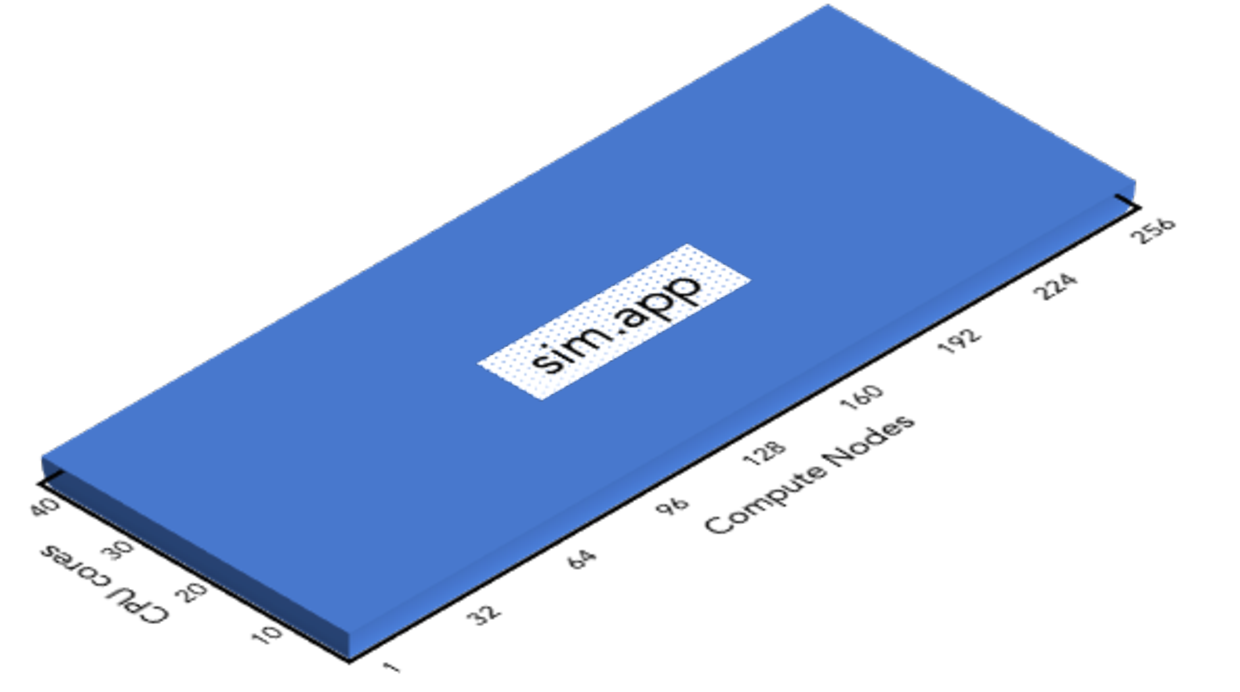
\includegraphics[width=1.1\textwidth]{projects/2.3.6-NNSA/2.3.6.02-LLNL-ATDM/Old}
            \label{fig:old}
         \end{minipage}}
  \hfill
   \subfloat[Emerging Paradigm] {
         \begin{minipage}[c][1\width]{
            0.48\textwidth}
            \centering
            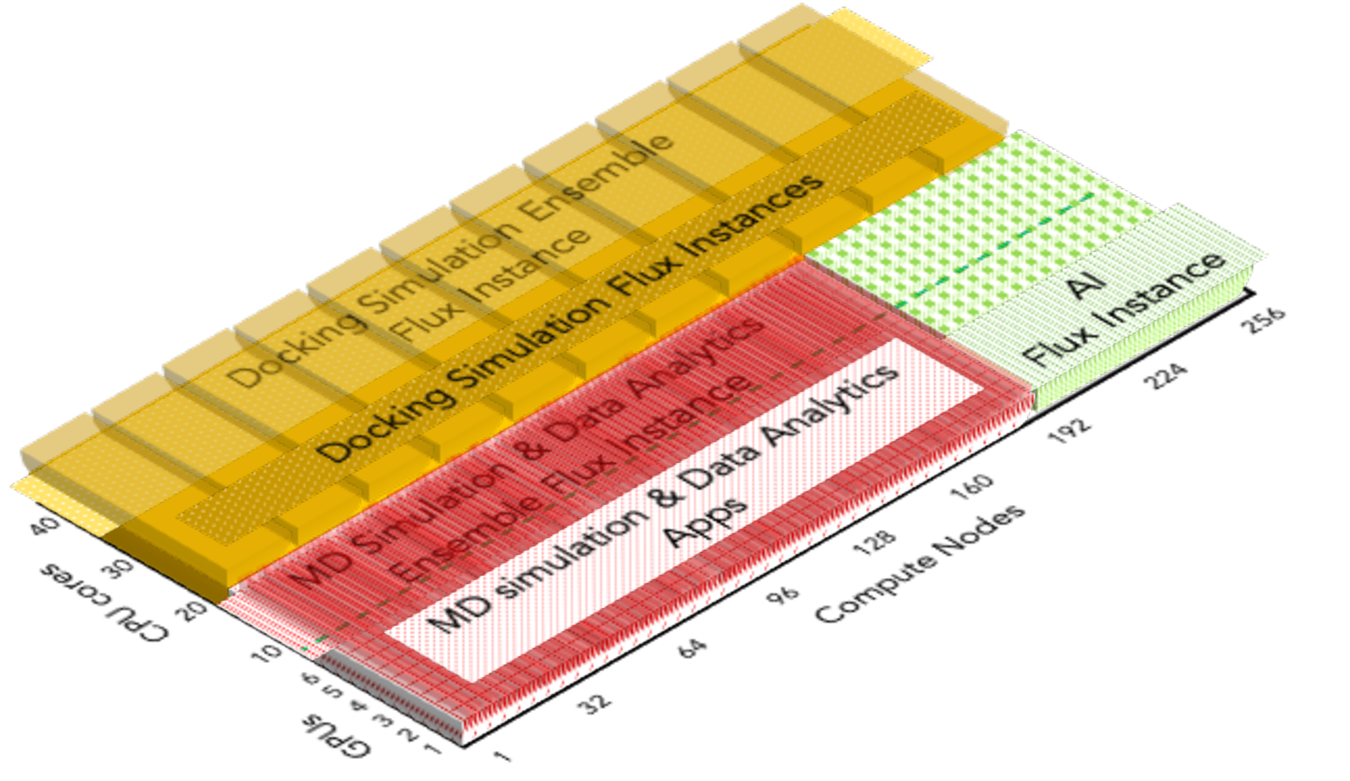
\includegraphics[width=1.1\textwidth]{projects/2.3.6-NNSA/2.3.6.02-LLNL-ATDM/New}
            \label{fig:new}
         \end{minipage}}
 \caption{An illustration of how the computing resources allocated
to a job---as granted by the HPC workload manager---differs between
conventional and emerging scientific workflows. The notional X-axes
depict the compute node IDs allocated to the job and Y-axes depict
the IDs of computing resources in each of these nodes. (a) The conventional paradigm
requires only a single parallel simulation application to run; (b) The emerging paradigm often requires many different types of tasks such as an ensemble of molecular dynamic (MD) parallel simulation applications and another ensemble of docking simulation applications along with in situ data analysis for the MD ensemble while these tasks are driven by an AI.}
 \label{fig:layout}
 \end{figure}
Figure~\ref{fig:layout} visually contrasts
the complexity of the conventional and
new or emerging HPC paradigms in terms of
how they utilize the resources allocated
by the system's workload manager.
Nearly all existing products were designed
when the workflows were much simpler
as shown in Figure~\ref{fig:old}.
Yet, these solutions have significant difficulties with
the emerging paradigm exemplified
by Figure~\ref{fig:new},
as well as with connecting and coordinating jobs.
These problems have led users to develop their own ad hoc
custom scheduling and resource management software or use tools
that perform only workflow management or only scheduling.
However, accomplishing sufficient job coordination without
first-class support from a workload manager
like Flux has already proven to be difficult
for either approach.
Perhaps more importantly, developing and maintaining ad hoc management
software---especially in this era of ever-evolving HPC hardware
architectures---has quickly become prohibitively expensive for
supercomputing application teams.
With Flux, a job script with multiple
tasks submitted on a heterogeneous HPC system
remains simple, requiring only a few more lines within
the script.

\subparagraph{AID}

Debugging a parallel code can be extremely difficult, and the most
exhaustive approaches for finding errors can require a large amount of
time to run.  For example, understanding all of the potential
interleavings of parallel threaded code requires combinatorial runtime
with respect to the number of threads.  It is not feasible to run this
type of analysis at all times.

Our strategy is to provide a continuum of debugging tools -- from the
lightweight tools like STAT, which require only seconds to run and gives
a high level overview of a code, to Archer, which requires lightweight
code instrumentation, to replay-based fuzzing tools like ReMPI and FLiT,
which run the code in a number of configurations to detect errors.  With
a suite of tools, we can enable developers to find the most common bugs
quickly, while still being able to detect deep, hard-to-find issues given
sufficient runtime and resources.

\subparagraph{Caliper}
Caliper is implemented as a C++ library and is linked with applications.
Application teams integrate it with their code by adding Caliper
annotations at the application level.  Contrast this with binary analysis
and DWARF line mappings used by most performance tools, which are
obtained automatically but increase tool complexity and are typically
not linked with the application for regular runs.

Applications, their libraries, physics modules, and even runtime systems
can be instrumented with Caliper and measured at the same time.  All of
these layers of the application stack provide additional context to
Caliper measurements and enable deeper analysis of the relationships
between different parts of the code.



%%%%%%%%%%%%%%%%%%%%%%%%%%%%%%%%%%%%%%%%%%%%%%%%%%%%%%%%%%%%%%%%%%%%%
\paragraph{Recent Progress} %\leavevmode \\
Recent progress includes developments in Spack; MFEM; RAJA, Umpire, and CHAI; Flux; AID; and Caliper.


\begin{figure}[tb]
\centering
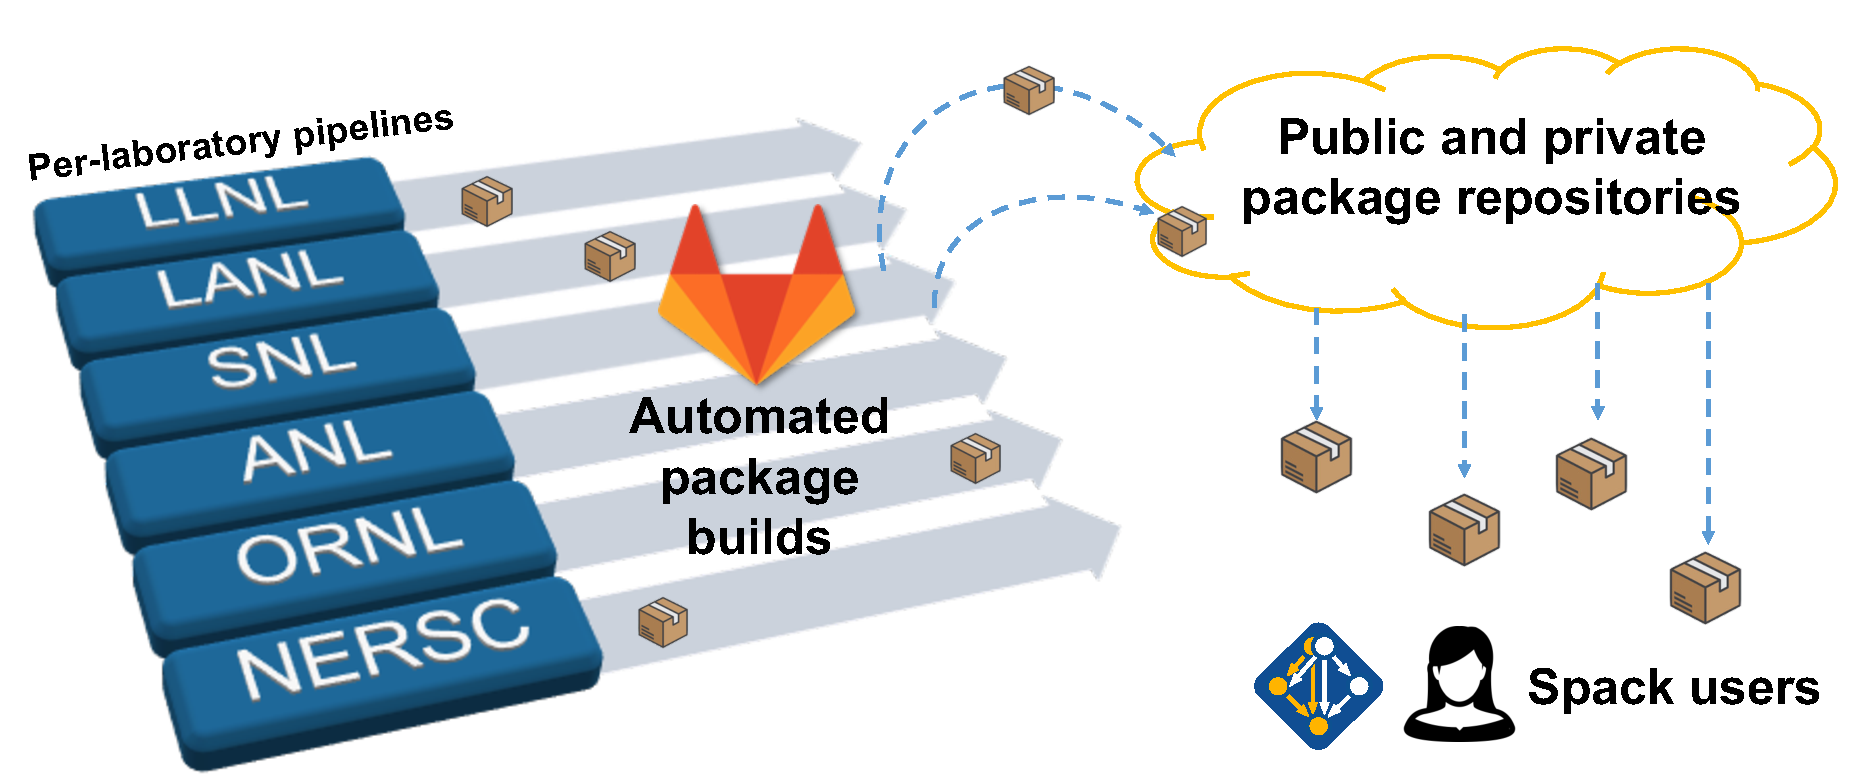
\includegraphics[width=.75\textwidth]{projects/2.3.6-NNSA/2.3.6.02-LLNL-ATDM/spack-pipelines.pdf}
\caption{Spack build pipelines at facilities will provide HPC-native binary builds for users.}
\label{figure:spack-build-pipeline}
\end{figure}


\subparagraph{Spack}
Spack 0.16.0 was released and replaced Spack's greedy concretizer algorithm with a much more aggressive solver based on Answer Set Programming.
There was also a major overhaul to smooth developer workflows and allow working directly on checked-out code in Spack.
Scalability of CI and binary cache creation in Spack was improved significantly (Figure~\ref{figure:spack-build-pipeline}).
GPU support was hardened in Spack, and CUDA and ROCm package superclasses were updated.


\begin{figure}[tb]
\centering
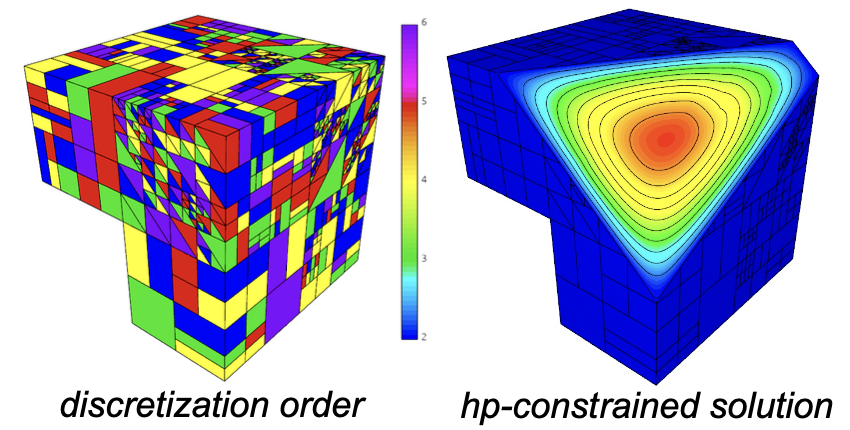
\includegraphics[width=.4\textwidth]{projects/2.3.6-NNSA/2.3.6.02-LLNL-ATDM/mfem-hp-refinement}
\caption{The MFEM team added support for variable order FEM spaces with general hp-refinement so higher order apps can better adapt to solutions.}
\label{figure:mfem-variable-order-fem}
\end{figure}

\subparagraph{MFEM}
Capabilities were added to MFEM for variable-order FEMs paces with general hp-refinement so HO apps can increase efficiency and better adapt to solutions (Figure~\ref{figure:mfem-variable-order-fem}).
ALE discretization improvements were implemented for compressible flow in BLAST, including significant improvements in mesh optimization methods, dynamic adaptive mesh refinement (AMR), and improved transfer between high-order and low-order-refined simulations.

\iffalse % Converted to table below. -STC.
\begin{figure}[htb]
\centering
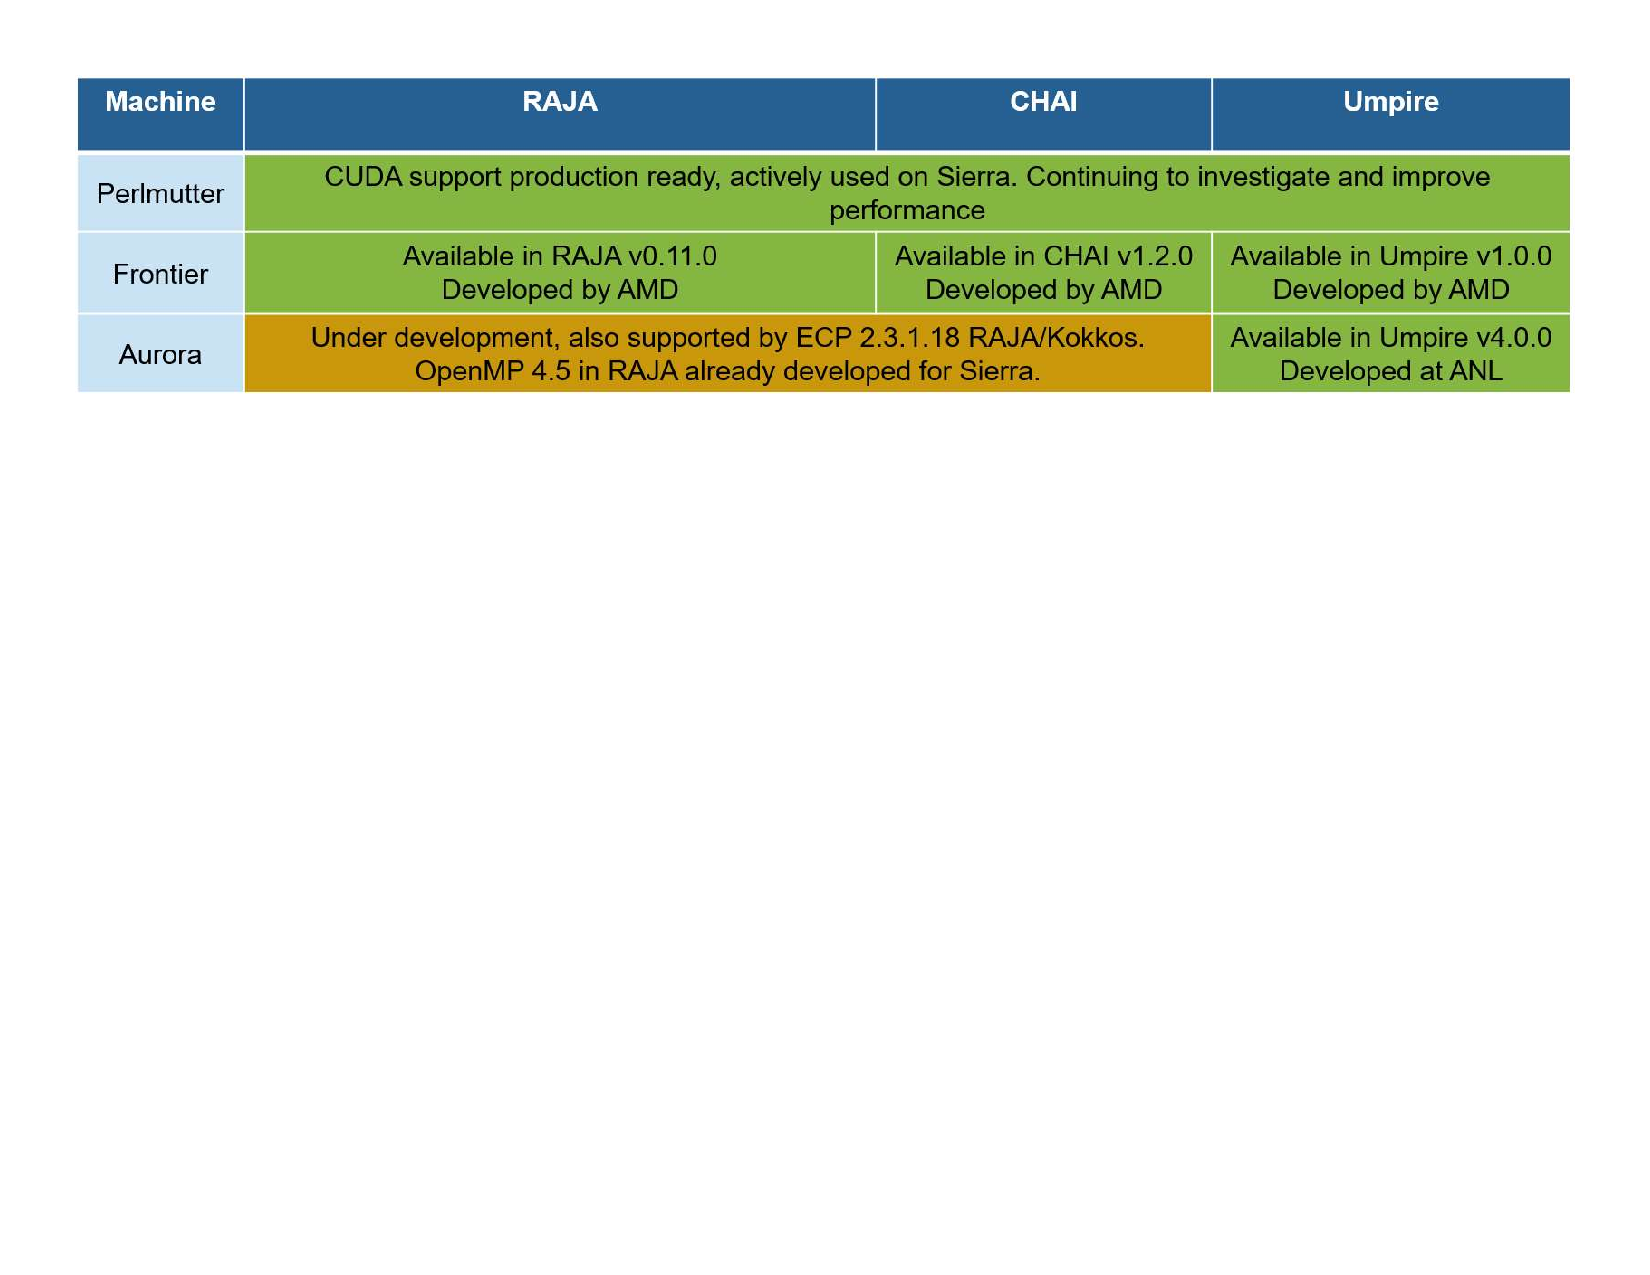
\includegraphics[width=\textwidth,trim={0 15cm 0 0},clip]{projects/2.3.6-NNSA/2.3.6.02-LLNL-ATDM/raja-umpire-chai-support}
\caption{Status of RAJA, Umpire, and CHAI support for exascale platforms.}
\label{figure:status-raja-umpire-chai}
\todo[inline]{Convert to table.}
\end{figure}
\fi

\begin{table}[h!]
\centering
\begin{tabular}{|>{\hspace{0pt}}m{0.12\linewidth}|>{\hspace{0pt}}m{0.25\linewidth}|>{\hspace{0pt}}m{0.25\linewidth}|>{\hspace{0pt}}m{0.25\linewidth}|}
\rowcolor{LightCyan}
\hline
\textbf{Machine} & \textbf{RAJA} & \textbf{CHAI} & \textbf{Umpire} \\ 
\hline
\textbf{Perlmutter} & \multicolumn{3}{>{\hspace{0pt}}m{0.80\linewidth}|}{CUDA support production ready, actively used on Sierra. Continuing to investigate and improve performance.} \\ 
\hline
\textbf{Frontier} & Available in RAJA v0.11.0. Developed by AMD. & Available in CHAI v1.2.0. Developed by AMD. & Available in Umpire v1.0.0. Developed by AMD. \\ 
\hline
\textbf{Aurora} & \multicolumn{2}{>{\hspace{0pt}}m{0.525\linewidth}|}{Under development, also supported by ECP 2.3.1.18 RAJA/Kokkos. OpenMP 4.5 in RAJA already developed for Sierra.} & Available in Umpire v4.0.0. Developed at Argonne. \\
\hline
\end{tabular}
\caption{Status of RAJA, Umpire, and CHAI support for exascale platforms.}
\label{table:status-raja-umpire-chai}
\end{table}

\subparagraph{RAJA, Umpire, and CHAI}

Table~\ref{table:status-raja-umpire-chai} shows the status of RAJA, Umpire, and CHAI support for exascale platforms.
The team updated support for AMD's HIP programming model and hardened support for El Capitan COE machines.
New versions of RAJA, Umpire, and CHAI with support for El Capitan COE machines were released.
HIP support was added to continuous integration using GitLab at LLNL.
Support for integration of Umpire into multiple ASC application codes continued.


\subparagraph{Flux}
%
Flux was the basis for a workflow of ECP ExaAM (ExaConstit) in improving its throughput by 4$\times$.
The Flux-based ML drug design workflow was part of an SC20 COVID-19 Gordon Bell finalist submission.
Optimization of Flux enabled the MuMMI workflow to run across the full scale of Summit at ORNL.
Support was added for exascale multitier storage in the Flux data-staging plugin and the Fluxion scheduler.

\subparagraph{AID}
%
We demonstrated that our new correctness tools (FLiT and FPChecker) can analyze large LLNL code, thereby discovering previously unknown issues in LLNL code. We also facilitated tools co-design via the El Capitan tools working group.

\subparagraph{Caliper}
We integrated the Caliper performance analysis tools into key LLNL applications. We also supported existing integration with MARBL via improvements to performance visualizations and analysis capabilities.


%%%%%%%%%%%%%%%%%%%%%%%%%%%%%%%%%%%%%%%%%%%%%%%%%%%%%%%%%%%%%%%%%%%%%
\paragraph{Next Steps} %\leavevmode \\
Next steps for each effort have already been identified and are described below.

\subparagraph{Spack}
 In FY22, the team will work to further improve Spack developer workflows and reproducibility and expand on the new concretizer to handle compiler and runtime complexity in the exascale stack.

\subparagraph{MFEM}
%
MFEM-based applications will be supported in their transition to exascale hardware.
The team will continue to engage with ATDM application work, develop mini-apps, and provide support.


\subparagraph{RAJA, Umpire, and CHAI}


GPU device capabilities will be expanded in Umpire, and the team will
investigate the use of Umpire as a GPU offload allocator for RAJA.
The team will continue to develop and deliver Umpire capabilities to applications in support of ASC milestone and user requirements, including interprocess shared memory to support shared on-node data and expanded functionality available inside GPU kernels.
The team will also continue interactions with El Capitan Center of Excellence (COE) partners to resolve performance and correctness issues identified as application users begin testing on early access hardware.


\subparagraph{Flux}
We will perform an end-to-end demonstration of HPE's Rabbit-based multitiered storage scheduling and management.
Support for Common Tools Interface (CTI)-based tool launching will be tuned to leverage HPE's proprietary code-development tools---Valgrind4HPC and ATP.
A Variorum-enabled power monitoring/capping subsystem, including power swing analysis, is also planned.
Finally, the team will respond to the emerging needs of existing and new advanced workflow customers.


\subparagraph{AID}
This effort will implement, evaluate, and harden a multilevel general-purpose GPU (GPGPU) debugging/code-correctness tool suite for early applications that run on Collaboration of Oak Ridge, Argonne, and Livermore (CORAL)-2 early access systems.

\subparagraph{Caliper}
Integrations of SPOT and Caliper within LLNL applications will continue. Tools will be expanded with more GPU and MPI measurement capabilities, and support, porting, and deployment of Caliper will continue.
